\chapter{Test bench}\label{ch:benchmark}
The model described in Section~\ref{sec:understanding} can be improved with different architectures and regularization methods. Besides that, training the model with new datasets can also lead to better results. In order to \emph{compare the performance} of these new models, a \emph{test bench} has been developed. In this chapter, the datasets employed to train the models, as well as the tools created to measure and visualize their performance, will be described.

\section{Datasets}\label{sec:datasets}
The digit classifier component is possible thanks to the data provided by the \emph{\gls{mnist} database} of handwritten digits. In the following sections, the pros and cons of using this database and some alternatives will be discussed.

\subsection{Original dataset}\label{subsec:MNIST}
\emph{\gls{mnist}} is a database of \emph{handwritten digits} formed by a training set, which contains~60000~samples, and a test set, containing~10000~samples~\cite{lecun-mnisthandwrittendigit-2010}. It's a \textit{remixed} and reduced version of the original \emph{NIST datasets}\footnote{\url{https://www.nist.gov/srd/nist-special-database-19}}. \gls{mnist} is a well-known benchmark for all kinds of \gls{ml} algorithms.

As may be seen in Figure~\ref{fig:mnist}, each sample of the \gls{mnist} database is a~28x28~pixels \emph{grayscale image} that contains a size-normalized and centered digit. While it may be useful for testing \gls{ml} algorithms, it's not enough to train a model that aims to solve a \emph{real-world task}, because the images are almost noiseless and the digits within them share similar orientation, position and size.
\begin{figure}
	\centering
	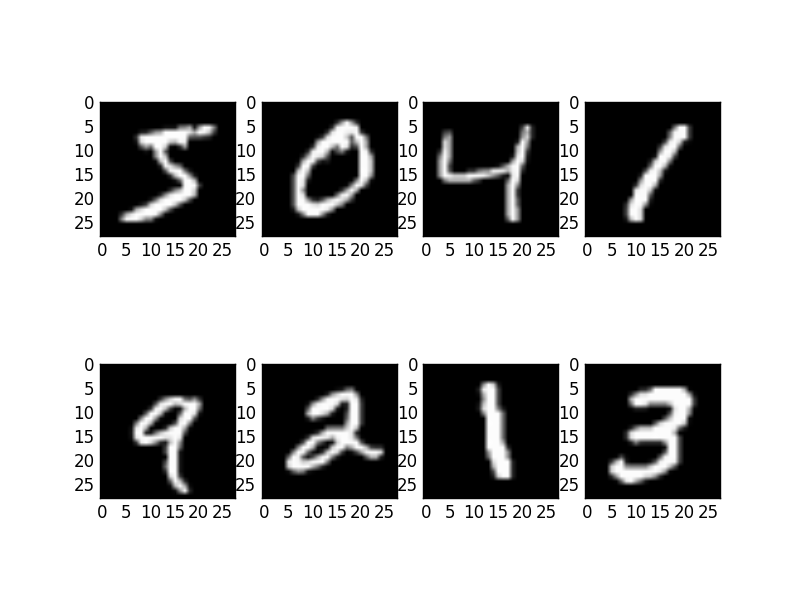
\includegraphics[width=12cm, keepaspectratio]{figures/mnist.png}
	\caption{Samples extracted from the MNIST database.}
	\label{fig:mnist}
\end{figure}

\subsection{Gradient images}\label{subsec:edge}
The first issue with \gls{mnist} database that must be addressed is that all the digits are white over a black background. In real world, the digits can be found written in several colors over different backgrounds and the datasets must resemble every possible combination. In order to achieve that generalization, the \emph{gradient of the images} has been calculated. The resultant samples are less dependent from the light and color conditions than the original ones, forcing the neural network to focus in the shape of the digits to classify them.

According to the study carried out by Nuria Oyaga\footnote{\url{http://jderobot.org/Noyaga-tfg\#Testing\_Neural\_Network}}, the operator that leads to better results is the \emph{Sobel filter}. This operator approximates the gradient of an image function~\cite{sonka1999image}, convolving the image with the following kernels to highlight horizontal and vertical edges, respectively:  
\begin{equation}\label{eq:sobel}
h_x = 
\begin{bmatrix}
1 & 2 & 1\\
0 & 0 & 0\\
-1 & -2 & -1
\end{bmatrix}
,\quad
h_y = 
\begin{bmatrix}
-1 & 0 & 1\\
-2 & 0 & 2\\
-1 & 0 & 1
\end{bmatrix}
\end{equation}
The absolute values of the resultant images, $x$ and $y$, are then added, obtaining the gradient image.

\subsection{Data augmentation}
The second problem that has been detected with \gls{mnist} is that the images are \emph{noiseless} and the digits are always centered with a scale and a rotation angle that are almost \emph{invariant}. However, the digit classifier has to deal with noisy images that can be randomly scaled, translated and/or rotated. In order to get a database with images that look like the ones that our application is going to work with, the \gls{mnist} database must be \emph{augmented}.

Two alternatives have been considered to solve this problem: real-time data augmentation provided by Keras and generating our own database.

\subsubsection{Real-time data augmentation with Keras}
Thanks to the \textit{.ImageDataGenerator()} method provided by Keras (see Section~\ref{subsec:utils}), the \gls{mnist} dataset can be augmented in \emph{real-time} during training. In order to cover most of the real cases, random rotation, translation and zooming has been applied to generate new samples. In addition to that, a Sobel filtering was also applied through a user-defined function. The samples generated by the following code can be seen in Figure~\ref{fig:aug_keras}.

\begin{lstlisting}
datagen = imkeras.ImageDataGenerator(
	                  zoom_range=0.2, rotation_range=20, width_shift_range=0.2, 
	                  height_shift_range=0.2, fill_mode='constant', cval=0,
	                  preprocessing_function=self.sobelEdges)
...	              
generator = datagen.flow(x, y, batch\_size=batch\_size)
\end{lstlisting}

\begin{figure}
	\centering
	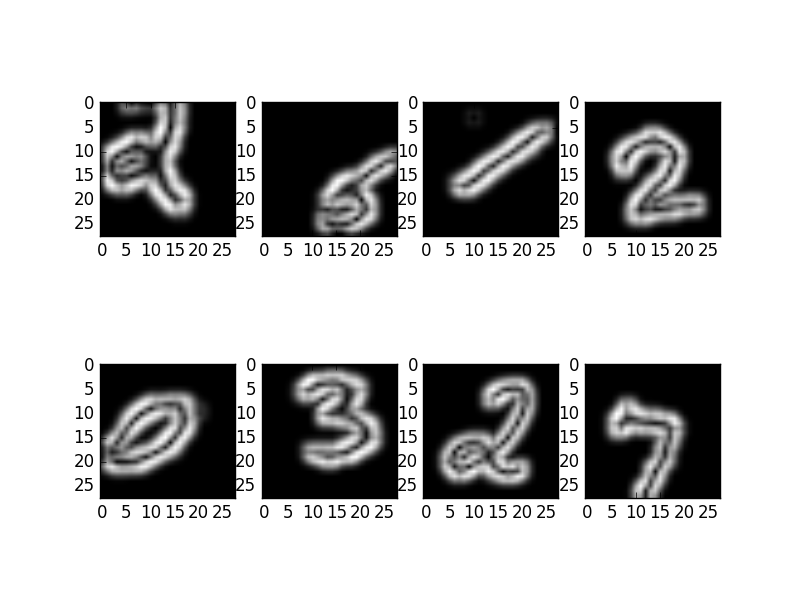
\includegraphics[width=12cm, keepaspectratio]{figures/aug_keras.png}
	\caption{Samples generated with Keras from MNIST database.}
	\label{fig:aug_keras}
\end{figure}

Besides these transformations, it's also necessary to simulate the \emph{noise} that may be present in real images. Keras generator doesn't support the addition of noise. For this purpose, Keras includes noise layers such as the \emph{GaussianNoise layer}, which adds Gaussian noise with a standard deviation distribution defined by the user. It's important to note that Keras treats noise layers as regularization methods that are only active during training time to avoid overfitting. In order to add noise to the generated samples, a GaussianNoise layer was established as the \emph{input layer} of the model.

\subsubsection{Handmade augmented datasets}\label{subsec:handmade}
The alternative to real-time data augmentation with Keras is building \emph{our own datasets} applying the previously mentioned transformations to the images. My mate Nuria Oyaga has build~5~new databases with two sets each one: training and validation\footnote{\url{http://jderobot.org/Noyaga-tfg\#Comparing_Neural_Network}}. These are the new databases: 
\begin{itemize}
	\item \textbf{Sobel}: \gls{mnist} database after applying the Sobel filter to every image.~48000~samples for training and~12000~samples for validation. 
	\item \textbf{0-1}: Same size than Sobel database. One transformed image per every Sobel database image. Sobel database images are replaced by the transformed ones.~48000~samples for training and~12000~samples for validation. 
	\item \textbf{1-1}: Double size than Sobel database. One transformed image per every Sobel database image. Both Sobel database images and the transformed images are included in the~1-1~database.~96000~samples for training and~24000~samples for validation. 
	\item \textbf{0-6}: Six times the size of Sobel database. Six transformed images per every Sobel database image. Sobel database images are replaced by the transformed ones.~288000~samples for training and~72000~samples for validation. 
	\item \textbf{1-6}: Seven times the size of Sobel database. Six transformed images per every Sobel database image. Both Sobel database images and the transformed images are included in the~1-6~database.~336000~samples for training and~84000~samples for validation. 
\end{itemize}

Besides that, the test dataset of the \gls{mnist} database (10000~samples) has been converted into a~\emph{1-6~test dataset} (70000~samples).

In Figure~\ref{fig:aug_nuria}, the first samples of every handmade dataset can be seen.

\begin{figure}
	\centering
	\begin{subfigure}{0.5\textwidth}
		\centering
		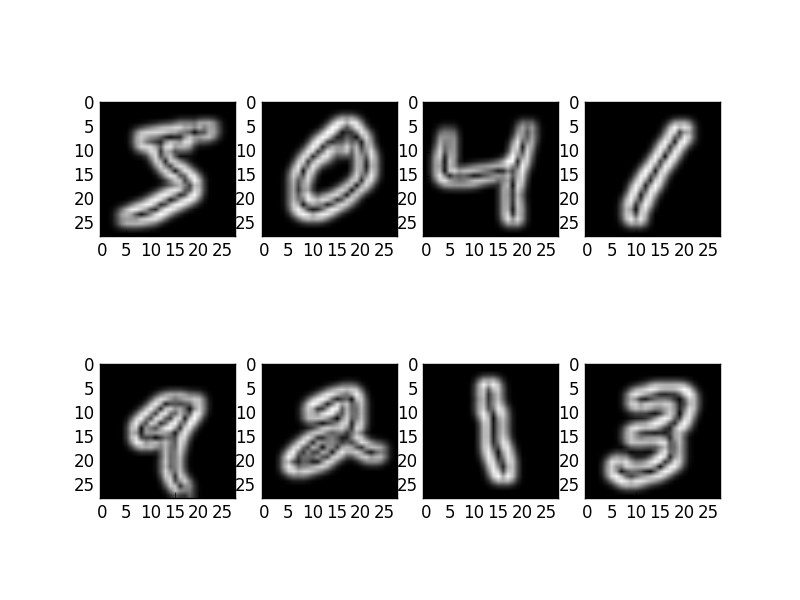
\includegraphics[width=1\linewidth]{figures/Sobel.png}
		\caption{}
	\end{subfigure}%
	\begin{subfigure}{0.5\textwidth}
		\centering
		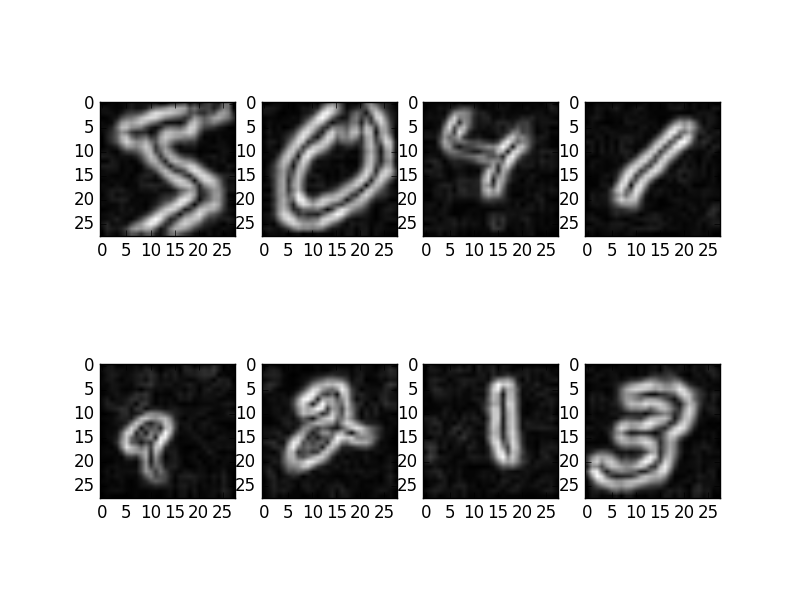
\includegraphics[width=1\linewidth]{figures/0-1.png}
		\caption{}
	\end{subfigure}
	\begin{subfigure}{0.5\textwidth}
		\centering
		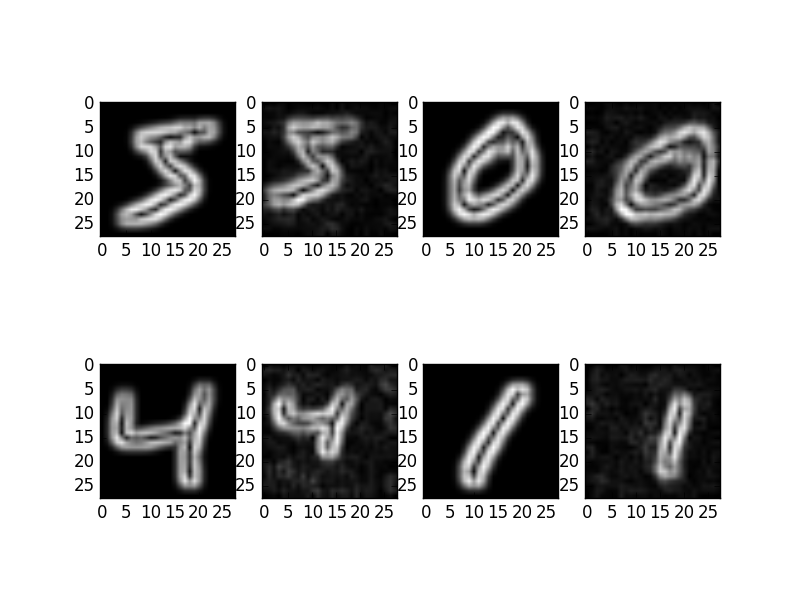
\includegraphics[width=1\linewidth]{figures/1-1.png}
		\caption{}
	\end{subfigure}%
	\begin{subfigure}{0.5\textwidth}
		\centering
		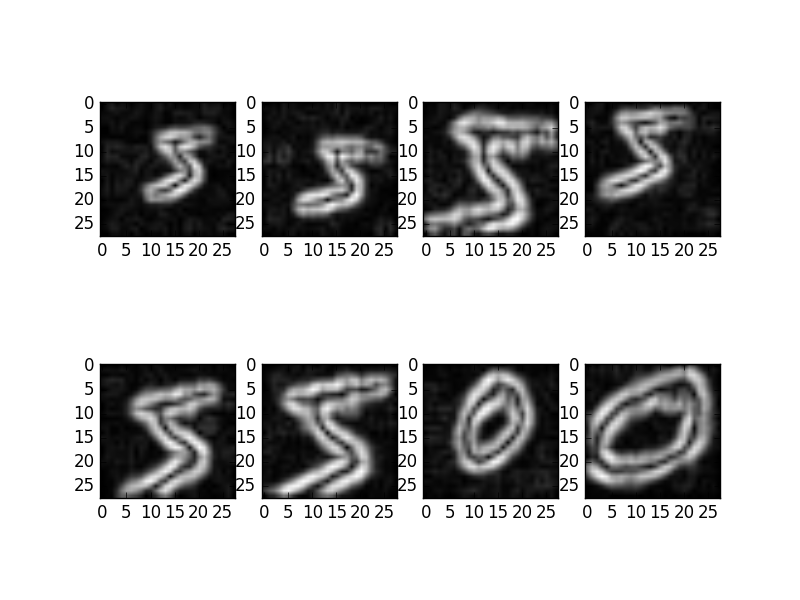
\includegraphics[width=1\linewidth]{figures/0-6.png}
		\caption{}
	\end{subfigure}
	\begin{subfigure}{0.5\textwidth}
		\centering
		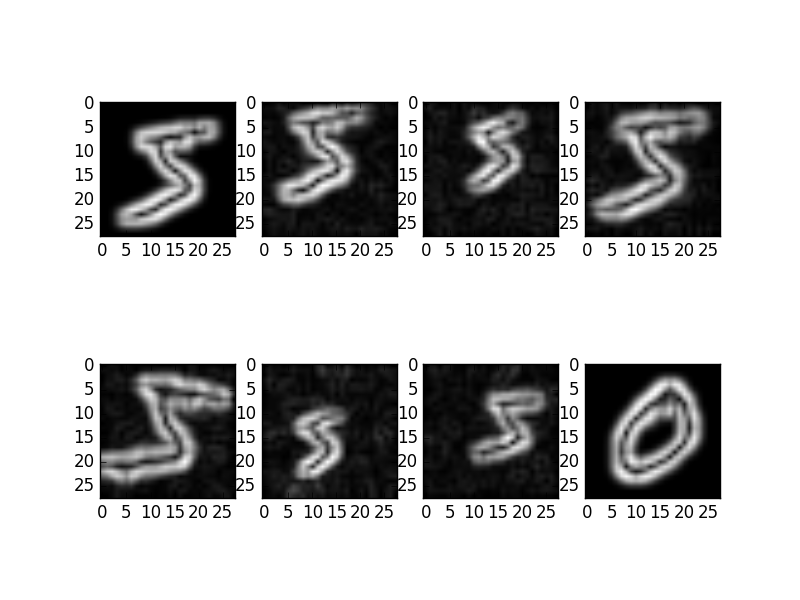
\includegraphics[width=1\linewidth]{figures/1-6.png}
		\caption{}
	\end{subfigure}
	\caption{First samples of handmade datasets: (a) Sobel; (b)~0-1; (c)~1-1; (d)~0-6~; (e)~1-6.}
	\label{fig:aug_nuria}
\end{figure}

\subsubsection{From LMDB to HDF5} \label{subsubsec:lmdb2hdf5}
These databases were initially built to feed a \emph{Caffe}~\cite{jia2014caffe} neural network. That's why they were saved as \emph{\gls{lmdb} files}\footnote{\url{http://www.lmdb.tech/doc/}}. In order to make it easier to feed the Keras model, the \gls{lmdb} databases have been converted into \emph{\gls{hdf5} files} (see Section~\ref{sec:hdf}). For this conversion, the script \emph{\textit{datasetconversion.py}} has been written.

\begin{itemize}
	\item \textbf{Reading the \gls{lmdb} database}. On one hand, the \gls{lmdb} library for Python\footnote{\url{https://lmdb.readthedocs.io/en/release/\#}} has been employed to open the database, initialize a cursor and iterate over each key-value pair in the database. On the other hand, \emph{Google's Protocol Buffers}\footnote{\url{https://developers.google.com/protocol-buffers/}} have been used to parse the data that were extracted from the database. ``With protocol buffers, you write a \textit{.proto} description of the data structure you wish to store. From that, the protocol buffer compiler creates a class that implements automatic encoding and parsing of the protocol buffer data with an efficient binary format"~\cite{protobuf}. Here can be seen the \textit{.proto} file that defines the data structure used by Caffe to store the \gls{mnist} database, as obtained from~\cite{lmdb_tutorial}: 
	
\begin{lstlisting}
package datum;
message Datum {
	optional int32 channels = 1;
	optional int32 height = 2;
	optional int32 width = 3;
	// the actual image data, in bytes
	optional bytes data = 4;
	optional int32 label = 5;
	// Optionally, the datum could also hold float data.
	repeated float float_data = 6;
	// If true data contains an encoded image that need to be decoded
	optional bool encoded = 7 [default = false];
}
\end{lstlisting}
	
	Thanks to the \textit{.proto} file, the compiler generates a Python module that contains the \emph{Datum class}. Datum class provides the \emph{\textit{.ParseFromString()} method}, which is employed to parse the image data. Here is the resulting code:

\begin{lstlisting}
# We initialize the cursor that we're going to use to access every
# element in the dataset.
lmdb_env = lmdb.open(sys.argv[1])
lmdb_txn = lmdb_env.begin()
lmdb_cursor = lmdb_txn.cursor()

x = []
y = []
nb_samples = 0

# Datum class deals with Google's protobuf data.
datum = datum.Datum()

if __name__ == '__main__':
	# We extract the samples and its class one by one.
	for key, value in lmdb_cursor:
		datum.ParseFromString(value)
		label = np.array(datum.label)
		data = np.array(bytearray(datum.data))
		im = data.reshape(datum.width, datum.height,
		datum.channels).astype("uint8")
	
		x.append(im)
		y.append(label)
		nb_samples += 1
		
		print("Extracted samples: " + str(nb_samples) + "\n")
	
	x = np.asarray(x)
	y = np.asarray(y)
\end{lstlisting}
	
	\item \textbf{Writing the \gls{hdf5} files}. Thanks to the \emph{h5py library\footnote{\url{http://www.h5py.org/}}} for Python, the data extracted from the \gls{lmdb} database has been stored into a \gls{hdf5} file with two datasets: label and data. The code can be seen in the following frame:	 
	\begin{lstlisting}
	f = h5py.File("../../Datasets/" + sys.argv[2] + ".h5", "w")
	
	# We store images.
	x_dset = f.create_dataset("data", (nb_samples, datum.width,
	datum.height, datum.channels), dtype="f")
	x_dset[:] = x
	
	# We store labels.
	y_dset = f.create_dataset("labels", (nb_samples,), dtype="i")
	y_dset[:] = y
	f.close()
	\end{lstlisting}
\end{itemize} 

\subsubsection{Conclusions}
After coding and testing both implementations for augmenting the database, it has been decided to use the \emph{handmade datasets}. While real-time data augmentation is really useful to avoid storing all the data that are needed for training, it makes harder to take a look into what is being fed to the network and reproduce results. Also, in this particular case, we are interested in \emph{comparing the performance} of neural networks built with different libraries, so they must be trained with the same datasets.

\section{Measuring performance}\label{sec:measuring}
The performance of the models will be evaluated using the \textit{CustomEvaluation} class and the measurements calculated with this class will be visualized using an Octave function. In this section, both of them will be described.

\subsection{\textit{CustomEvaluation} class}
\emph{\textit{CustomEvaluation} class} is totally independent from Keras. It calls functions that measure the performance of the model during test and/or training time and saves them into a file which is compatible with Octave.
\begin{itemize}
	\item \textbf{Obtaining the measurements}. The user provides the real labels and the probability distribution of the predicted ones. Log loss, accuracy, precision, recall and a confusion matrix are computed. These functions are defined in Section~\ref{sec:skoctave} and Section~\ref{subsec:models}.
	\item \textbf{Storing results}. \textit{CustomEvaluation} class stores the results in a \emph{Python dictionary}. Additionally, it can store the \emph{learning curves} if \textit{training} option is set. In the following section, the Keras callback employed to build the learning curves will be discussed.
	\item \textbf{Python-Octave \textit{translation}}. For this task, the \emph{SciPy library}\footnote{\url{https://docs.scipy.org/doc/scipy-0.18.1/reference/index.html}} has been used. It provides the \textit{.savemat()} method that saves Python dictionaries into Matlab \textit{.mat} files, which are also compatible with Octave (see Section~\ref{sec:skoctave}).
\end{itemize}

Here's a usage example:
\begin{lstlisting}
if training == "n":
	measures = CustomEvaluation(y_test, y_proba, training)
else:
	train_loss = learning_curves.loss
	train_acc = learning_curves.accuracy
	val_loss = validation.history["val_loss"]
	val_acc = validation.history["val_acc"]
	results = CustomEvaluation(y_test, y_proba, training, train_loss,
	train_acc, val_loss, val_acc)

results_dict = results.dictionary()
results.log(results_dict)
\end{lstlisting}

\subsubsection{\textit{LearningCurves} callback} \label{subsubsec:learningcurves}
During training time, Keras automatically saves into a \textit{.History()} object (see Section~\ref{subsec:callbacks}) the validation results obtained after every epoch. It's interesting to face these validation results with the ones obtained after every batch during training.

\emph{\textit{LearningCurves}} is a custom Keras callback that has been coded to save the accuracy and loss obtained after each batch into Python lists. The code below shows how it works.
\begin{lstlisting}
class LearningCurves(keras.callbacks.Callback):
''' LearningCurve class is a callback for Keras that saves accuracy
and loss after each batch.
'''    

def on_train_begin(self, logs={}):
	self.loss = []
	self.accuracy = []

def on_batch_end(self, batch, logs={}):
	self.loss.append(float(logs.get('loss')))
	self.accuracy.append(float(logs.get('acc')))
\end{lstlisting}

\subsection{Octave function}\label{subsec:octave-func}
Now that all the data have been collected, they have to be properly displayed. The function \emph{\textit{visualization.m}} has been written to address this issue. It takes as its only argument the path to the \textit{.mat} file that has been generated with the \textit{CustomEvaluation} class and plots the results as shown in Figure~\ref{fig:benchmark}. Additionally, it prints them to the standard output.

\begin{figure}
	\centering
	\begin{subfigure}{1\textwidth}
		\centering
		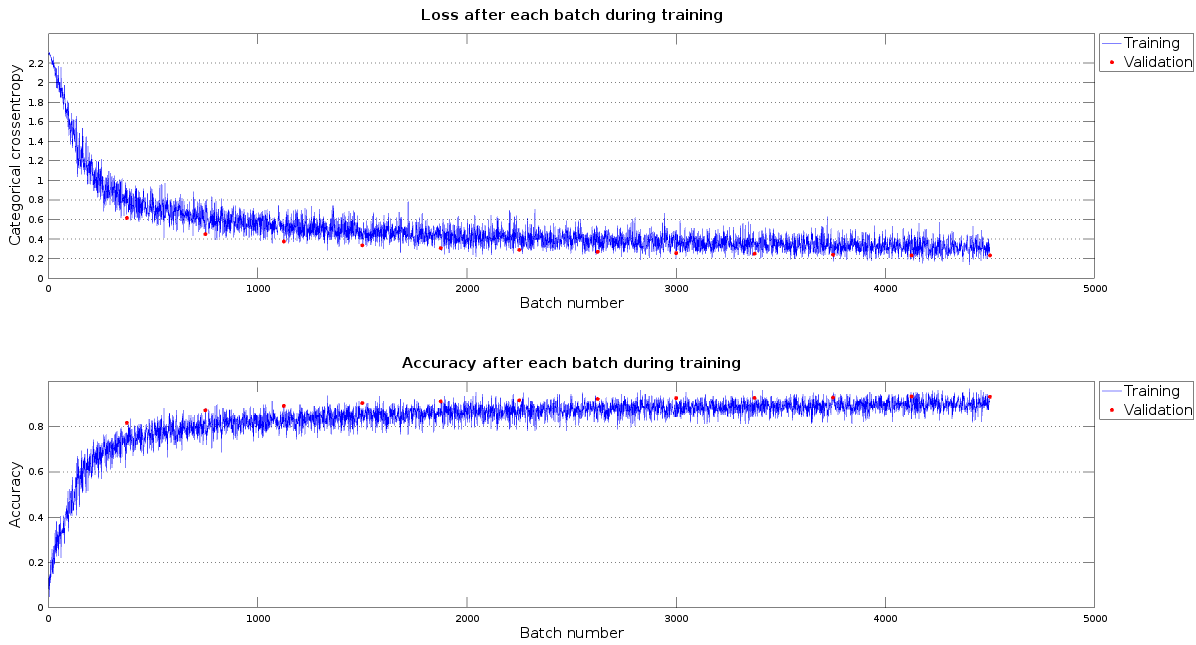
\includegraphics[width=1\linewidth]{figures/learning_curves.png}
		\caption{}
	\end{subfigure}
	\begin{subfigure}{0.5\textwidth}
		\centering
		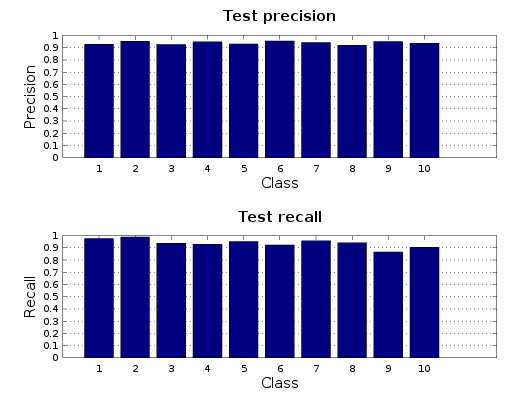
\includegraphics[width=1\linewidth]{figures/prec_rec.png}
		\caption{}
	\end{subfigure}%
	\begin{subfigure}{0.5\textwidth}
		\centering
		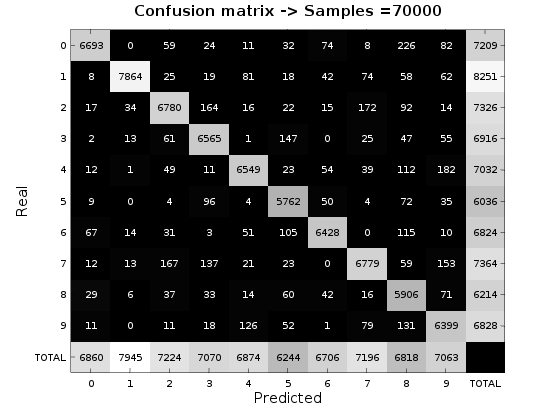
\includegraphics[width=1\linewidth]{figures/conf_mat.png}
		\caption{}
	\end{subfigure}
	\caption{Parameters displayed by \textit{visualization.m}: (a) learning curves; (b) precision and recall; (c) confusion matrix.}
	\label{fig:benchmark}
\end{figure}

\section{Convolutional layers visualization}\label{sec:visualization}
\glspl{cnn} are well-known by their ability of learning \emph{image features}. The weights of a convolutional layer are arranged like \emph{a set of filters}, each of which learns to identify a certain visual feature~\cite{cs231n}. As the filter is convolved with the input image, it generates an \emph{activation map} that will tell us how that particular filter reacts to that image. In other words, the activation map will tell us whether a certain feature is present in the image or not.

In order to understand how the Keras model is learning to classify the digits, the \emph{\textit{layer\_visualization.py}} script has been written. This script allows the user to display the filters that are learned in every convolutional layer of the model and their resulting activation maps.

\subsection{Filters}
Keras provides a list containing every \emph{layer object} in the model through the attribute \textit{model.layers}. Layer objects properties can be accessed thanks to the \textit{layer.get\_config()} method. Since convolutional layers in Keras are named with the prefix \textit{conv2d}, it is possible to iterate over the names of the layers looking for that prefix to find the convolutional ones, as it is shown in the code below.

\begin{lstlisting}
for i, layer in enumerate(self.model.layers):
	if layer.get_config()["name"][:6] == "conv2d":
...
\end{lstlisting}

Once the convolutional layers have been found, their \emph{filters} are accessed through the \textit{layer.get\_weigths()} method. The matrices of weights returned by this method are reshaped to improve readability. The code that performs these operations can be seen in the following frame:

\begin{lstlisting}
shape = layer.get_weights()[0].shape
weights = layer.get_weights()[0].reshape(shape[2], shape[0],
                                              shape[1], shape[3])
\end{lstlisting}

Finally, the filters are plotted thanks to the \emph{Matplotlib library}\footnote{\url{https://matplotlib.org/}} for Python. The shape and the maximum/minimum values of the weights are printed to the standard output. An example of how the filters are plotted can be seen in the following chapter in Figure~\ref{fig:filters}

\subsection{Activation maps}
The output of each convolutional layer is formed by as many \emph{activation maps} as filters the layer has. In order to get the values of these activation maps, \emph{truncated versions} of the original model are generated, as it is shown in Figure~\ref{fig:truncated}. When a prediction is made with these truncated models, they output the activation maps that correspond to their last layer. The code which obtains the activation maps can be seen in the follwing frame:
\begin{lstlisting}
truncated = Model(inputs=self.model.inputs,
                    outputs=layer.output)
activations = truncated.predict(self.im)
\end{lstlisting}

\begin{figure}
	\begin{subfigure}{0.5\textwidth}
		\centering
		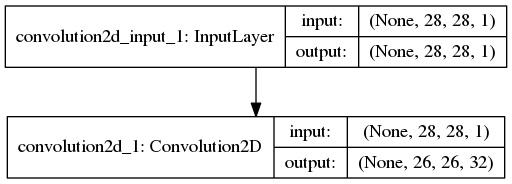
\includegraphics[width=0.9\linewidth]{figures/1stconvarch.png}
		\caption{}
	\end{subfigure}
	\begin{subfigure}{0.5\textwidth}
		\centering
		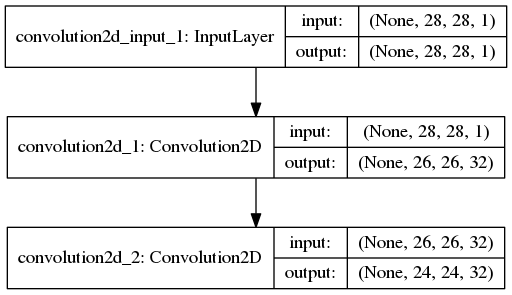
\includegraphics[width=0.9\linewidth]{figures/2ndconvarch.png}
		\caption{}
	\end{subfigure}
	\caption{Truncated versions of the model: (a) one convolutional layer; (b) two convolutional layers}
	\label{fig:truncated}
\end{figure}

The activation maps are plotted using the Matplotlib library as well, and their shape and maximum/minimum values are also printed to the standard output. An example of how the activation maps are plotted can be seen in the following chapter in Figure~\ref{fig:activation_maps}.
